\documentclass[a4paper,12pt]{article}

% Language and encoding
\usepackage[french]{babel}
\usepackage[utf8]{inputenc}
\usepackage[T1]{fontenc}
\usepackage{amsmath} 
\usepackage{booktabs}
\usepackage{xcolor}
\usepackage{hyperref}
\usepackage{qrcode}
\usepackage{xcolor}

\usepackage{array}
\usepackage{caption}


\usepackage{amssymb} % fournit \mathbb
% ou \usepackage{amsfonts}



% Page layout and spacing
\usepackage[margin=2.5cm]{geometry}
\usepackage{setspace}
\usepackage{float}


% Graphics and figures
\usepackage{graphicx}
\graphicspath{ {./images/} }
\usepackage{tikz}
\usepackage{tikzpagenodes}

% Hyperlinks and references
\usepackage{hyperref}

\hypersetup{
    hidelinks
}


% Tables
\usepackage{booktabs} % For \toprule, \midrule, and \bottomrule
\usepackage{array}    % For custom column formatting
\usepackage{longtable} % If long tables are needed
\usepackage{multirow} % If multirow is needed in tables

% % Bibliography
% \usepackage{biblatex}
% \addbibresource{references.bib} % Adjust the bibliography file name

% For placeholder text
\usepackage{blindtext}

% Additional utilities for tables
\usepackage{tabularx} % If width-adjustable columns are needed
\usepackage{colortbl} % If color in tables is required


% Informations du rapport
\newcommand{\titre}{Rain in Australia | Kaggle}
\newcommand{\UE}{UAE}
\newcommand{\sujet}{Sujet du rapport}
\newcommand{\enseignant}{Pr.Anass Belcaid}
\newcommand{\eleves}{
    Qassiri Adnane \\
    Nadi Yasser \\
    Jadli said }
\setlength{\parskip}{1.4\baselineskip}  % Set line spacing for paragraphs
\begin{document}

% Page de garde
\begin{titlepage}
    \centering
    \includegraphics[width=1\textwidth]{logos/Logo-ENSA.png} % Insérer le logo ici
    \vspace{1cm}
    {\LARGE \textsc{Deep Learning : Project Repport} \par} 
    \hrulefill \\[0.4cm]
    {\huge \textbf{Satellite Single Image Super
Resolution using Deep Learining
techniques} \par} % Titre principal
    \hrulefill \\[1.5cm]
    
    \vspace{1.2cm}
 
    \begin{minipage}{0.5\textwidth}
        \Large
        \raggedright
        \textbf{Élèves :} \\ % Liste des étudiants
        \eleves
    \end{minipage}
    \hfill
    \begin{minipage}{0.4\textwidth}
        \Large
        \raggedleft
        \textbf{Enseignant :} \\ % Nom de l'enseignant
        \enseignant
    \end{minipage}

    \vfill
    {\Large \today \par} % Date du jour
\end{titlepage}

% \renewcommand\thesection{\roman{section}}
\setlength{\parskip}{1.5ex}  % Augmente l'espace entre les paragraphes

\newpage

\tableofcontents
\newpage


\section{Introduction}
\subsection{Motivation}
High-resolution (HR) satellite imagery plays a crucial role in Earth observation by enabling detailed analysis of surface features and spatial patterns. The availability of fine-grained visual information allows for more accurate interpretation of land use, infrastructure, vegetation, and environmental changes, which is essential for informed decision-making in many scientific and industrial domains.

HR satellite imagery has become a key asset in several application areas. In urban planning, it supports tasks such as infrastructure development, traffic analysis, and monitoring urban expansion. In agriculture, high-resolution images enable precise crop monitoring, yield estimation, irrigation management, and early detection of plant stress or diseases. Similarly, in environmental monitoring, HR imagery is widely used to track deforestation, desertification, water resources, and the impacts of climate change, contributing to more effective environmental protection and policy planning.

Despite its importance, the acquisition of high-resolution satellite imagery faces significant physical and economic limitations. The deployment and maintenance of high-resolution satellites involve substantial costs, including satellite construction, launch, and operation. Additionally, physical constraints such as sensor limitations, orbital parameters, atmospheric conditions, and limited revisit frequency restrict the availability and temporal coverage of HR data. As a result, high-resolution imagery is often scarce, expensive, or unavailable for continuous monitoring, particularly in large-scale or resource-constrained scenarios. These limitations motivate the exploration of alternative approaches, such as computational enhancement techniques, to improve the utility of low-resolution satellite imagery while reducing dependence on costly HR data acquisition.


\subsection{Problem statement}

Single Image Super-Resolution (SISR) refers to the problem of reconstructing a high-resolution (HR) image from a single low-resolution (LR) observation by recovering spatial details lost during the satellite image acquisition process. In the context of satellite imagery, this problem is particularly challenging due to sensor resolution limitations, atmospheric effects, orbital constraints, and the complex spatial structures present in both natural and urban environments.

Formally, SISR for satellite imagery can be defined as the estimation of a mapping function that relates a low-resolution image to its corresponding high-resolution representation. Let $I^{LR} \in \mathbb{R}^{H \times W \times C}$ denote a low-resolution satellite image and $I^{HR} \in \mathbb{R}^{4H \times 4W \times C}$ its high-resolution counterpart, where $H$ and $W$ represent the spatial dimensions and $C$ denotes the number of spectral channels. The objective is to estimate a function $f(\cdot)$, parameterized by $\theta$, such that:
\begin{equation}
I^{HR} = f(I^{LR}; \theta)
\end{equation}

The mapping function $f$ is generally unknown and must be approximated using available observations or prior knowledge. In this work, the super-resolution task is restricted to a $4\times$ scale factor, which represents a practical compromise between reconstruction complexity and spatial detail enhancement. This setting is commonly adopted in satellite imaging applications, as it provides a significant improvement in spatial resolution while remaining feasible for real-world deployment.


\section{Dataset, Patching, and Performance Metrics}

\subsection{Dataset Description}

We use the \textbf{4× Satellite Image Super-Resolution} dataset, provided on Kaggle, which is specifically designed for supervised super-resolution of satellite imagery.  
The dataset consists of co-registered pairs of high-resolution (HR) and low-resolution (LR) satellite images covering identical geographic regions.

The HR images have a spatial resolution of approximately 0.5 meters per pixel, while the corresponding LR images have a resolution of 2 meters per pixel, resulting in a spatial upscaling factor of 4× between LR and HR images.

\begin{itemize}
    \item \textbf{High-Resolution (HR) images:} Stored in directories such as \texttt{HR\_0.5m/}, provided as GeoTIFF files with fine spatial details.
    \item \textbf{Low-Resolution (LR) images:} Stored in directories such as \texttt{LR\_2m/}, each LR image is spatially aligned with a corresponding HR image.
    \item \textbf{Dataset size:} The dataset contains a total of 360 paired images, with one LR image and one HR image per pair.
\end{itemize}

All image pairs are geo-aligned, meaning that corresponding pixels in LR and HR images represent the same geographic locations. This alignment enables pixel-wise supervised learning for super-resolution tasks.




\subsection{Image Dimensions and Patch-Based Preprocessing}

The original high-resolution (HR) satellite images have large spatial dimensions of approximately $3000 \times 3000$ pixels.  
Training super-resolution models directly on full-resolution images is computationally expensive and inefficient in terms of GPU memory usage. To overcome this limitation, we adopt a \textbf{patch-based preprocessing and training strategy}, which is a standard and effective practice in computer vision and image super-resolution.

In this approach, each large image is decomposed into smaller, fixed-size patches that can be processed independently by the neural network. An image patch represents a localized region of the image and contains sufficient contextual information to learn spatial patterns such as edges, textures, and structural details.

Specifically, we extract paired low-resolution (LR) and high-resolution (HR) patches with sizes defined according to the upscaling factor:
\begin{itemize}
    \item Each LR patch has a spatial size of $32 \times 32$ pixels.
    \item The corresponding HR patch has a spatial size of $128 \times 128$ pixels, consistent with the 4× super-resolution scale factor.
\end{itemize}


  \begin{figure}[H]
    \centering
    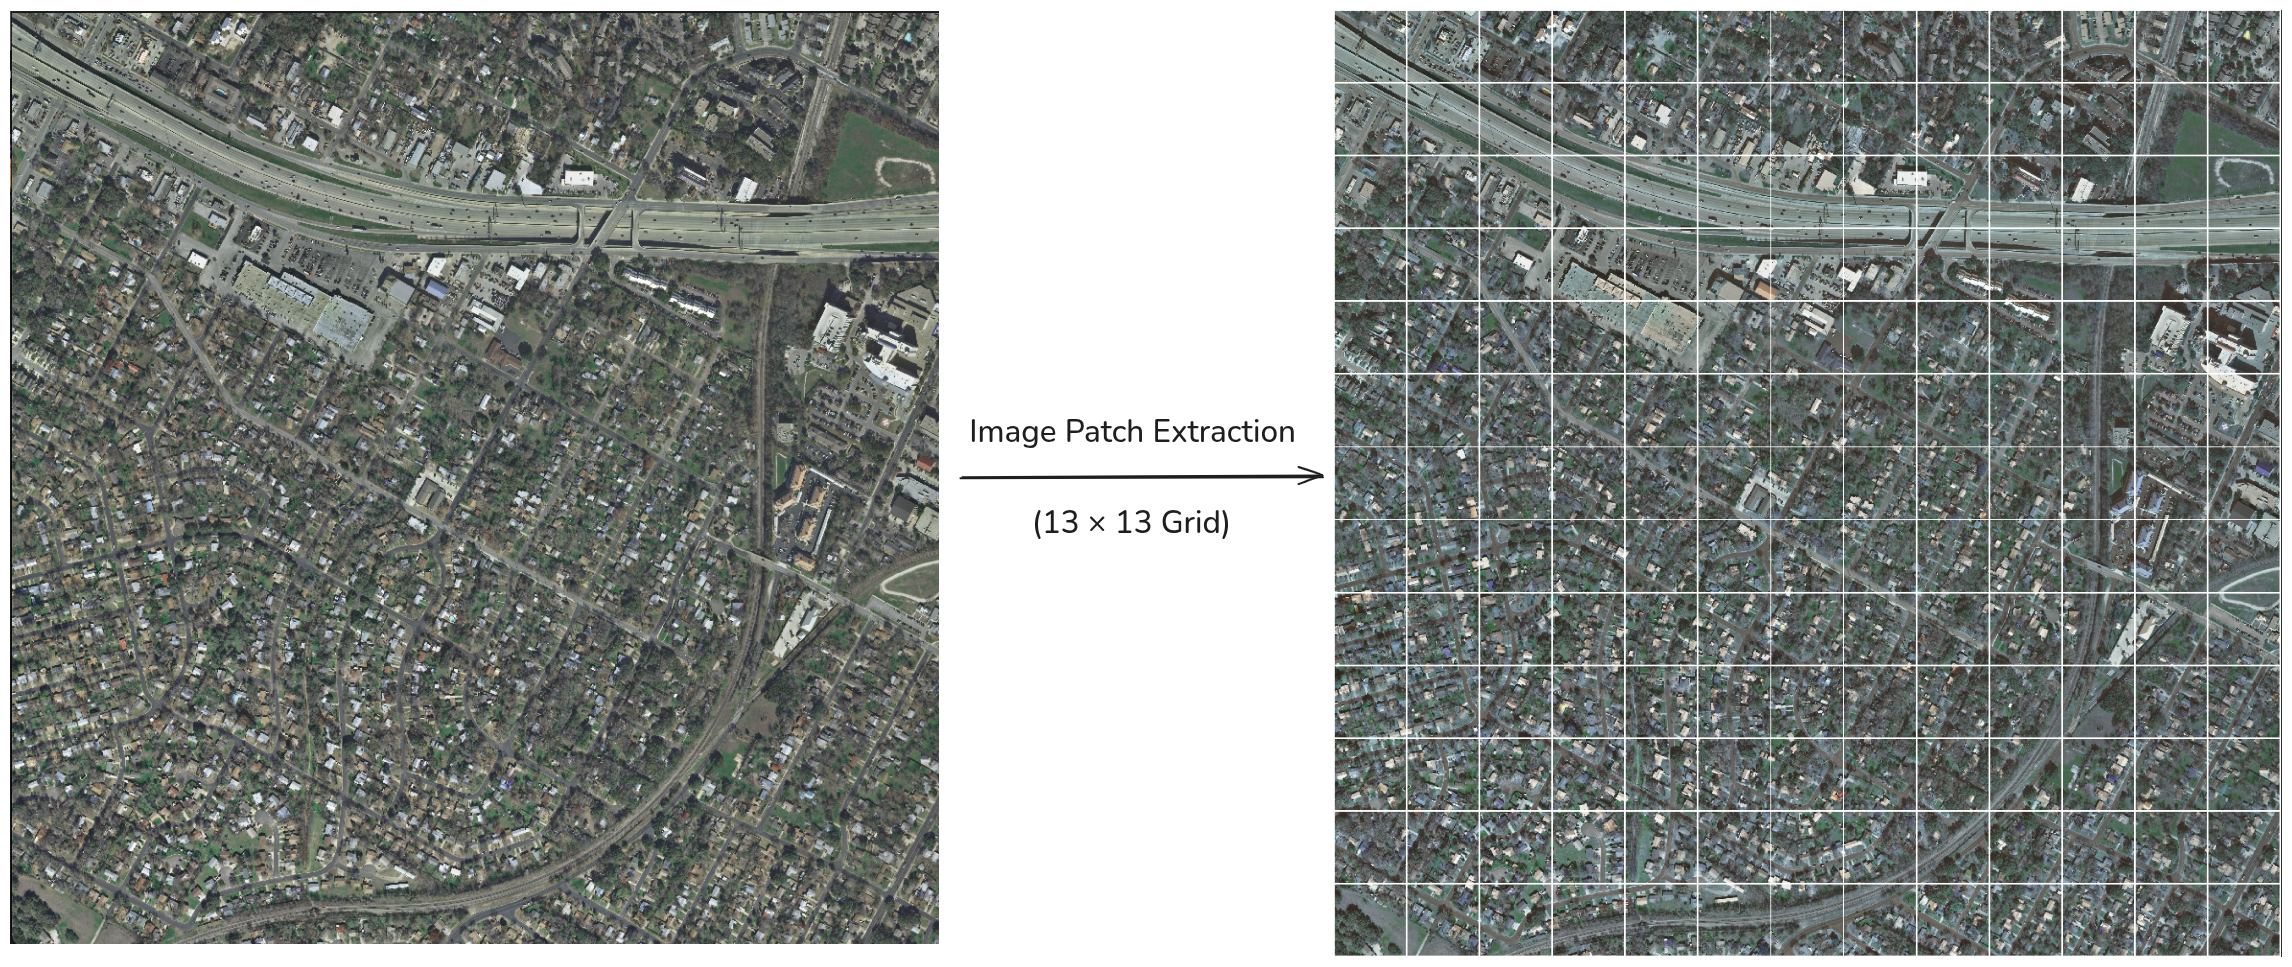
\includegraphics[width=1\textwidth]{Samples/image patche extraction.png}
    \caption{Data Samples After Patching}
    \label{fig:faster_rcnn}
   \end{figure}


Patch extraction is performed using a sliding window with zero overlap, ensuring complete coverage of the original images while avoiding redundant samples. Each LR patch is mapped to its corresponding HR patch using spatially consistent coordinates, forming paired training samples $\{(x_i, y_i)\}$ for supervised learning.

The use of patch-based training provides several important advantages: it significantly reduces memory consumption, enables efficient batch processing, increases the effective number of training samples, and encourages the model to learn robust local spatial correlations. As a result, this strategy improves training stability and enhances the generalization capability of the super-resolution model to unseen geographic regions and image content.


\subsection{Samples vizualisation}
  \begin{figure}[H]
    \centering
    \includegraphics[width=1\textwidth]{Samples/samples_viz.png}
    \caption{Data Samples After Patching}
    \label{fig:faster_rcnn}
   \end{figure}
\subsection{Evaluation Metrics}

To quantitatively assess the quality of the reconstructed high-resolution images, we employ several widely used evaluation metrics in image super-resolution. These metrics jointly evaluate pixel-wise fidelity, structural similarity, and perceptual quality.

\subsubsection{Peak Signal-to-Noise Ratio (PSNR)}

Peak Signal-to-Noise Ratio (PSNR) is a full-reference metric that measures the pixel-wise reconstruction accuracy between the predicted high-resolution image $\hat{y}$ and the ground-truth image $y$.  
Higher PSNR values indicate lower reconstruction error and better numerical fidelity.

\[
\mathrm{PSNR}(y,\hat{y}) = 10 \log_{10} \left( \frac{MAX_I^2}{\mathrm{MSE}(y,\hat{y})} \right),
\]

where $MAX_I$ denotes the maximum possible pixel value and $\mathrm{MSE}(\cdot)$ represents the mean squared error between the two images.  
Although PSNR is widely adopted due to its simplicity and interpretability, it does not always correlate well with human visual perception, particularly for high-frequency textures.

\subsubsection{Structural Similarity Index Measure (SSIM)}

The Structural Similarity Index Measure (SSIM) evaluates perceptual similarity by comparing local patterns of luminance, contrast, and structural information between the reconstructed image $\hat{y}$ and the reference image $y$.

\[
\mathrm{SSIM}(y,\hat{y}) =
\frac{(2\mu_y \mu_{\hat{y}} + C_1)(2\sigma_{y\hat{y}} + C_2)}
{(\mu_y^2 + \mu_{\hat{y}}^2 + C_1)(\sigma_y^2 + \sigma_{\hat{y}}^2 + C_2)}.
\]

Here, $\mu_y$ and $\mu_{\hat{y}}$ denote mean intensities, $\sigma_y^2$ and $\sigma_{\hat{y}}^2$ represent variances, and $\sigma_{y\hat{y}}$ is the covariance between the two images.  
SSIM correlates better with human visual perception than PSNR, as it explicitly models structural information.

\subsubsection{Learned Perceptual Image Patch Similarity (LPIPS)}

Learned Perceptual Image Patch Similarity (LPIPS) is a perceptual similarity metric designed to align closely with human judgments of image quality.  
Instead of relying on pixel-wise differences, LPIPS computes distances between deep feature representations extracted from multiple layers of pretrained convolutional neural networks (e.g., VGG or AlexNet).

Formally, given two images $y$ and $\hat{y}$, LPIPS measures the weighted $\ell_2$ distance between their normalized feature maps:
\[
\mathrm{LPIPS}(y,\hat{y}) = \sum_{l} w_l \left\| \phi_l(y) - \phi_l(\hat{y}) \right\|_2^2,
\]
where $\phi_l(\cdot)$ denotes the feature activations at layer $l$ and $w_l$ are learned weights that emphasize perceptually important features.

LPIPS is particularly well-suited for super-resolution tasks, as it is sensitive to semantic content, texture realism, and high-frequency details that are often poorly captured by PSNR and SSIM.  
Lower LPIPS values indicate greater perceptual similarity between the reconstructed and ground-truth images, making it a complementary metric for evaluating visual quality beyond numerical accuracy.

Together, PSNR, SSIM, and LPIPS provide a comprehensive evaluation framework that balances numerical fidelity, structural consistency, and perceptual realism in super-resolved images.




\section{Models Development}


% ==============================================




\subsection{SRCNN: Super-Resolution Convolutional Neural Network}

The Super-Resolution Convolutional Neural Network (SRCNN) represents the first
successful deep learning-based approach applied to the problem of single-image
super-resolution. Proposed by Dong et al., this model introduces an end-to-end
learning formulation that directly learns the mapping between a low-resolution
image and its high-resolution counterpart, without relying on complex pipelines
based on handcrafted heuristics.


\subsubsection{Global Architecture of SRCNN}

SRCNN is a fully convolutional network composed of three successive layers, each
corresponding to a conceptual stage of the super-resolution process:

\begin{itemize}
    \item patch extraction and representation,
    \item nonlinear mapping between low- and high-resolution representations,
    \item final reconstruction of the high-resolution image.
\end{itemize}

The network contains neither pooling layers nor fully connected layers, which
allows the spatial resolution to be preserved throughout the entire processing
pipeline.

    
    \begin{figure}[H]
        \centering
        \includegraphics[width=1\textwidth]{Architectures/SRCNN.png}
        \caption{Global architecture of the SRCNN model}
        \label{fig:srcnn_architecture}
    \end{figure}
    


\subsubsection{Network Layers and Mathematical Modeling}

\paragraph{First layer: Patch extraction and representation}

The first layer applies a set of convolutional filters to extract local features
such as edges, textures, and patterns. This operation is defined as:

\begin{equation}
F_1(Y) = \max(0, W_1 * Y + B_1)
\end{equation}

where \( W_1 \) denotes the convolutional filters, \( B_1 \) the associated
biases, and \( * \) the convolution operation.  
The ReLU activation function introduces nonlinearity and contributes to training
stability.

\paragraph{Second layer: Nonlinear mapping}

The second layer performs a nonlinear transformation between the low-resolution
representation and an intermediate representation associated with the
high-resolution image:

\begin{equation}
F_2(Y) = \max(0, W_2 * F_1(Y) + B_2)
\end{equation}

This stage can be interpreted as a neural generalization of sparse coding, but
implemented in a fully feed-forward manner and optimized through learning.

\paragraph{Third layer: Reconstruction}

The final layer aggregates the learned representations in order to reconstruct
the final high-resolution image:

\begin{equation}
F(Y) = W_3 * F_2(Y) + B_3
\end{equation}

This operation replaces the manual aggregation mechanisms used in classical
approaches and enables a direct and coherent reconstruction of the image.



% ===================================================
\subsection{SRResnet: Super Resolution Residual Network}
    After the introduction of SRCNN, which demonstrated the effectiveness of
  convolutional neural networks for single image super-resolution, further re-
  search focused on improving reconstruction accuracy by increasing network
  depth. However, directly deepening SRCNN-style architectures leads to trai-
  ning difficulties such as vanishing gradients and slow convergence. To address
  these limitations, SRResNet(site) was proposed as a more advanced deep lear-
  ning architecture for SISR. It adopts the residual learning framework introdu-
  ced in ResNet(site), allowing the network to learn residual mappings instead
  of directly predicting the high-resolution image from the low-resolution in-
  put. By learning only the difference between the interpolated LR image and
  its HR counterpart, SRResNet simplifies the learning task and enables the
  stable training of much deeper networks. This residual design significantly
  improves reconstruction performance while preserving fine image details, making SRResNet a substantial improvement over the original SRCNN model.
  \subsubsection{Residual Block}
  The residual block is the fundamental building unit of SRResNet and is designed to facilitate the learning of high-frequency image details in deep networks. Rather than directly learning a mapping between consecutive feature representations, each residual block estimates a residual function that captures the difference between its input and output. Let $\mathbf{x}_l$ denote the input feature map at layer $l$. The output of the residual block, $\mathbf{x}_{l+1}$, is defined as
\[
\mathbf{x}_{l+1} = \mathbf{x}_l + \mathcal{F}(\mathbf{x}_l),
\]
where $\mathcal{F}(\mathbf{x}_l)$ represents the nonlinear transformation learned by the convolutional layers within the block. The identity skip connection enables direct information and gradient propagation across layers, which improves training stability and convergence when stacking many residual blocks. This residual learning formulation allows SRResNet to employ significantly deeper architectures than SRCNN while effectively enhancing texture reconstruction and edge sharpness.

    \begin{figure}[H]
        \centering
        \includegraphics[width=0.8\textwidth]{Architectures/residual_block.png}
        \caption{residual block}
        \label{fig:residual-block}
    \end{figure}

  \subsubsection{Sub-pixel convolution }
  The sub-pixel convolution layer in SRResNet serves as the upsampling mechanism that transforms low-resolution feature maps into high-resolution outputs. Unlike traditional interpolation methods, sub-pixel convolution learns the upsampling process through data-driven training. It works by applying convolutional operations to increase the number of channels, then rearranging these channels into spatial dimensions via a process known as period shuffling. Specifically, SRResNet employs two such layers to achieve a 4× upscaling factor
    \begin{figure}[H]
        \centering
        \includegraphics[width=1.1\textwidth]{Architectures/sub-pixel.png}
        \caption{Sub-pixel convolution}
        \label{fig:sub-pixel-convolution}
    \end{figure}
  \subsubsection{Overall Architecture of SRResNet}

  Building upon residual blocks and sub-pixel convolution, the overall architecture of SRResNet follows a fully convolutional pipeline composed of feature extraction, deep residual mapping, and image reconstruction stages. The network first extracts low-level features from the interpolated low-resolution input, which are then progressively refined through a stack of residual blocks. The resulting feature maps are finally passed to the sub-pixel upsampling module to generate the super-resolved image. This hierarchical design integrates efficient upsampling with deep residual learning, leading to substantial performance improvements over SRCNN.

  \begin{figure}[H]
    \centering
    \includegraphics[width=1\textwidth]{Architectures/srresnet-architecture.png}
    \caption{Architecture of srresnet}
    \label{fig:srresnet-architecture}
   \end{figure}



% ==============================================






\subsection{EDSR: Enhanced Deep Residual Network}

Following SRResNet, which demonstrated the effectiveness of residual connections
for single-image super-resolution, the \textbf{Enhanced Deep Residual Network
(EDSR)} proposes a refined revision of the residual architecture in order to
better adapt it to low-level image reconstruction tasks. Introduced by Lim et
al., EDSR does not challenge the residual learning principle itself, but rather
builds upon a critical analysis of architectural choices inherited from
classification networks, some of which are not well suited for super-resolution.

Unlike SRResNet, which largely adopts the classical ResNet structure, EDSR is
characterized by two fundamental design choices: the complete removal of batch
normalization layers and the introduction of a \textit{residual scaling}
mechanism to stabilize the training of very deep and wide networks.

\subsubsection{Enhanced Residual Blocks}

Similar to SRResNet, EDSR relies on a sequence of residual blocks designed to
facilitate the learning of high-frequency details. Each block consists of two
$3 \times 3$ convolutional layers separated by a ReLU activation function and
connected through a direct residual connection. However, EDSR completely removes
the batch normalization layers present in SRResNet.

This design choice is motivated by the observation that batch normalization tends
to constrain the dynamic range of activations, which is detrimental to
super-resolution tasks where pixel-level accuracy and intensity preservation are
critical. By removing these layers, EDSR allows the network to preserve richer
luminance and texture information while significantly reducing memory
consumption. This optimization enables the training of much wider models without
compromising numerical stability.

    \begin{figure}[H]
        \centering
        \includegraphics[width=0.5\textwidth]{Architectures/Residual_Block.png}
        \caption{Structure of an optimized residual block in the EDSR model}
        \label{fig:edsr_resblock}
    \end{figure}


\subsubsection{Residual Scaling and Training Stability}

One of the main evolutions introduced by EDSR compared to SRResNet lies in the
significant increase in model capacity, particularly through the use of a large
number of filters, reaching up to 256 channels per convolutional layer. However,
this increase leads to numerical instability during training if left
uncontrolled.

To address this issue, EDSR introduces a \textit{residual scaling} mechanism,
which consists of weighting the output of each residual block by a constant
factor $\alpha$, empirically set to $0.1$:
\[
\mathbf{y} = \mathbf{x} + \alpha \cdot F(\mathbf{x})
\]

This factor limits the magnitude of the corrections introduced by each residual
block, thereby stabilizing gradient backpropagation during training. Residual
scaling thus enables the effective exploitation of very deep and wide
architectures while maintaining stable convergence and high performance.


\subsubsection{Overall Architecture of the EDSR Model}

The overall architecture of EDSR follows the same general design introduced by
SRResNet, relying on a fully convolutional organization with residual blocks and
a learned upsampling module at the end of the network. The differences between
the two models mainly stem from the internal optimization of residual blocks and
the training stabilization mechanisms presented earlier, while the global
pipeline structure remains unchanged.

    \begin{figure}[H]
        \centering
        \includegraphics[width=0.7\textwidth]{Architectures/edsr_architecture.png}
        \caption{Overall architecture of the EDSR model}
        \label{fig:edsr_architecture}
    \end{figure}





% ==============================================




\subsection{ESRGAN: Enhanced Super Resolution GAN}
ESRGAN is the enhanced version of the \textbf{SRGAN (cite)}. The authors of ESRGAN aimed to improve super-resolution performance by modifying both the \textbf{model architecture} and the \textbf{loss functions}.

\subsubsection{GAN: Generative Adversarial Network}
A \textbf{Generative Adversarial Network (GAN)} consists of two neural networks trained in an \textbf{adversarial manner}: a \textbf{generator} $G$ and a \textbf{discriminator} $D$. The generator aims to produce \textbf{synthetic samples} that resemble real data, while the discriminator attempts to \textbf{distinguish real samples from generated ones}.

Given a real image $x \sim p_{data}(x)$ and a noise vector $z \sim p_z(z)$, the generator produces a fake sample $G(z)$, and the discriminator outputs a \textbf{probability} $D(x)$ indicating whether the input is real. The GAN training objective is defined as a \textbf{minimax optimization problem}:
\vspace{0.3cm}
\[
\min_G \max_D \; \mathbb{E}_{x \sim p_{data}(x)}[\log D(x)] + \mathbb{E}_{z \sim p_z(z)}[\log (1 - D(G(z)))]
\]

During \textbf{adversarial training}, the discriminator learns to improve its \textbf{classification accuracy}, while the generator learns to \textbf{fool the discriminator} by generating more realistic samples. In \textbf{super-resolution tasks} such as ESRGAN, the generator uses a \textbf{low-resolution image} as input, and the adversarial loss encourages the generation of \textbf{visually realistic high-resolution images}.

  \begin{figure}[H]
    \centering
    \includegraphics[width=0.8\textwidth]{Architectures/GAN-architecture.png}
    \caption{Architecture of GANs}
    \label{fig:faster_rcnn}
   \end{figure}
\subsubsection{Adversarial Loss in ESRGAN}
To improve perceptual realism, ESRGAN adopts an adversarial loss based on the \textbf{Relativistic Average GAN (RaGAN) (cite)} framework. Unlike standard GANs, where the discriminator predicts the probability of an image being real or fake independently, RaGAN estimates the probability that a real image appears more realistic than a generated one.

Let $x_r \sim p_{data}$ denote a real high-resolution image and $x_f = G(I_{LR})$ a generated image. The relativistic discriminator output is defined as:
\[
D_{Ra}(x_r, x_f) = \sigma\left(D(x_r) - \mathbb{E}_{x_f}[D(x_f)]\right)
\]
\[
D_{Ra}(x_f, x_r) = \sigma\left(D(x_f) - \mathbb{E}_{x_r}[D(x_r)]\right)
\]
where $D(\cdot)$ denotes the discriminator output before activation and $\sigma(\cdot)$ is the sigmoid function.

The adversarial loss for the generator is then expressed as:
\[
\mathcal{L}_{adv}^{G} =
-\mathbb{E}_{x_r}[\log(1 - D_{Ra}(x_r, x_f))]
-\mathbb{E}_{x_f}[\log(D_{Ra}(x_f, x_r))]
\]

This relativistic formulation provides more informative gradients and improves training stability, leading to sharper and more realistic textures.

In ESRGAN, the generator is optimized using a \textbf{weighted combination} of adversarial loss, \textbf{perceptual (content) loss (cite)}, and \textbf{pixel-wise $L_1$ loss (cite)}. The complete generator objective is defined as:
\[
\mathcal{L}_{G} =
\lambda_{adv}\mathcal{L}_{adv}^{G}
+ \lambda_{perc}\mathcal{L}_{content}
+ \lambda_{L1}\mathcal{L}_{L1}
\]
where $\lambda_{adv}$, $\lambda_{perc}$, and $\lambda_{L1}$ control the contribution of each loss term.

\subsubsection{Networks Architecture}
The architecture of ESRGAN is based on SRGAN(site) with key modifications to improve perceptual quality. The main enhancement is the introduction of \textbf{Residual-in-Residual Dense Blocks (RRDB) (cite resnet and densenet)}, which combine multi-level residual learning and dense connections while removing Batch Normalization.

\paragraph{Main Components}

\subparagraph{1. Generator Network}
The generator transforms a low-resolution image into a high-resolution output. It consists of an initial convolution layer, a stack of \textbf{RRDB blocks} for deep feature extraction, followed by upsampling layers and final convolution layers to produce the super-resolved image.

\begin{figure}[H]
    \centering
    \includegraphics[width=1\textwidth]{Architectures/Gen_archi.png}
    \caption{ESRGAN | Architecture of the Generator}
    \label{fig:esrgan_generator}
\end{figure}

\subparagraph{2. Residual-in-Residual Dense Blocks (RRDB)}
RRDB blocks are the fundamental components of the generator. They integrate dense connections and nested residual learning to facilitate training of very deep networks while preserving image details, without using Batch Normalization.

\begin{figure}[H]
    \centering
    \includegraphics[width=1\textwidth]{Architectures/RRDB-archi.png}
    \caption{ESRGAN | Architecture of RRDB}
    \label{fig:rrdb_arch}
\end{figure}

\subparagraph{3. Discriminator Network}
The discriminator is a convolutional network designed to distinguish real high-resolution images from generated ones. ESRGAN employs a \textbf{relativistic discriminator}, which compares the relative realism between real and generated images to guide adversarial training.

\begin{figure}[H]
    \centering
    \includegraphics[width=1\textwidth]{Architectures/Disc_diagram-Page-1.drawio (3).png}
    \caption{ESRGAN | Architecture of the Discriminator}
    \label{fig:esrgan_discriminator}
\end{figure}



\subsection{MSFSSR: Multi-Scale and Frequency-Separated Super-Resolution Network}

\subsubsection{Motivation and Positioning}

Recent advances in Single Image Super-Resolution (SISR) have been dominated by deep residual learning approaches such as EDSR, which focus on maximizing reconstruction accuracy, and adversarial models such as ESRGAN, which emphasize perceptual quality. Despite their success, both approaches present limitations when applied to fidelity-critical domains such as satellite and remote sensing imagery.

EDSR processes features within a unified representation space and does not explicitly model frequency components, which limits its ability to separately handle structural and textural information. In contrast, ESRGAN relies on adversarial training, which may introduce visually plausible but physically incorrect details, leading to hallucinated textures.

To address these limitations, we propose \textbf{MSFSSR}, a \textit{Multi-Scale and Frequency-Separated Super-Resolution} network. The proposed model aims to enhance feature representation through multi-scale residual learning, explicitly separate low- and high-frequency information, and preserve reconstruction fidelity without adversarial training. This design enables a balance between accuracy, stability, and structural faithfulness.

\subsubsection{Multi-Scale Residual Block Definition}

To enrich early feature representations, MSFSSR uses a \textbf{Multi-Scale Residual Block (MSRB)}(site). Unlike conventional residual blocks that employ a single convolutional kernel size, the MSRB captures spatial information at multiple receptive fields using parallel convolutional operations.
  \begin{figure}[H]
    \centering
    \includegraphics[width=0.8\textwidth]{Architectures/MSRB.jpeg}
    \caption{Architecture of MSRB}
    \label{fig:MSRB-architecture}
   \end{figure}
Each MSRB consists of parallel $3 \times 3$ and $5 \times 5$ convolutions followed by feature concatenation and shared processing. A second multi-scale interaction stage further refines the combined features, which are then fused using a $1 \times 1$ convolution to reduce channel dimensionality. Residual scaling is applied to ensure stable training of deep networks.

Formally, given an input feature map $x_l$, the output of the MSRB is defined as:
\begin{equation}
x_{l+1} = x_l + \alpha \cdot \mathcal{F}_{\text{ms}}(x_l),
\end{equation}
where $\mathcal{F}_{\text{ms}}(\cdot)$ denotes the multi-scale transformation and $\alpha$ is a residual scaling factor.

This structure enables the network to simultaneously capture fine-grained textures and broader spatial context, providing enriched features for subsequent frequency-aware learning.

\subsubsection{Frequency-Separated Learning}

\subsubsection*{Frequency Separation}

Following multi-scale feature enhancement, MSFSSR explicitly decomposes feature representations into low-frequency (LF) and high-frequency (HF) components. This design is motivated by the observation that smooth structures and fine details exhibit distinct characteristics and should be processed differently.

The low-frequency branch consists of a sequence of residual blocks that model large-scale structures and smooth regions, ensuring global consistency. In contrast, the high-frequency branch begins with a fixed Laplacian convolution, acting as a high-pass filter that emphasizes edges and fine details. The extracted high-frequency features are subsequently refined using residual blocks.

The Laplacian kernel is non-learnable, introducing an explicit inductive prior that enforces edge-aware feature extraction and improves training stability.
  \begin{figure}[H]
    \centering
    \includegraphics[width=0.8\textwidth]{Architectures/laplacianfilter.jpeg}
    \caption{image after Laplacian filter}
    \label{fig:Laplacian-Img}
   \end{figure}

\subsubsection*{Feature Fusion}

The outputs of the low- and high-frequency branches are concatenated along the channel dimension and fused using a $1 \times 1$ convolution. This fusion operation learns adaptive weighting between frequency components while reducing the feature dimensionality.

By jointly exploiting complementary frequency information, the proposed fusion strategy enables faithful reconstruction of both structural content and fine details.

\subsubsection{Overall Architecture}

The overall architecture of MSFSSR follows a structured and efficient pipeline. First, shallow feature extraction is performed using a $3 \times 3$ convolution. The extracted features are then enhanced by one or more Multi-Scale Residual Blocks. Subsequently, the enriched features are processed through parallel low- and high-frequency branches to explicitly model different frequency components.

After frequency fusion, the resulting feature maps are upsampled using sub-pixel convolution (PixelShuffle) to achieve the desired resolution. Global residual learning is employed by adding a bicubic-upsampled version of the input image to the network output, allowing the model to focus on learning high-frequency residuals. Finally, a refinement block operating in the RGB space further improves local consistency and suppresses reconstruction artifacts.

Through the combination of multi-scale spatial modeling, explicit frequency separation, and residual learning, MSFSSR achieves stable and high-fidelity super-resolution reconstruction without adversarial training.

  \begin{figure}[H]
    \centering
    \includegraphics[width=1\textwidth]{Architectures/MSFSSR.jpeg}
    \caption{General architecture of MSFSSR}
    \label{fig:MSFSSR-arch}
   \end{figure}


   

\section{Training Details}

\subsection{Objective Functions and Optimization}
Following the description of the model architectures, this section outlines the loss functions and optimization strategy employed during training, in line with commonly used approaches in the literature.
\subsubsection{Loss Functions}

Loss functions employed during training aim to measure discrepancies at both low-level and perceptual feature levels.

\subparagraph{L1 Reconstruction Loss}
The L1 loss measures the absolute difference between the predicted output $\hat{y}$ and the corresponding ground-truth target $y$ at the pixel level. 
It is formulated as:
\begin{equation}
\mathcal{L}_{\text{L1}} = \frac{1}{N} \sum_{i=1}^{N} \left| \hat{y}_i - y_i \right|,
\end{equation}
where $N$ denotes the total number of pixels.

Due to its reduced sensitivity to outliers compared to the L2 loss, the L1 loss is widely used in reconstruction tasks and is known to encourage sharper and more stable results.

\subparagraph{Perceptual (Content) Loss}
Pixel-wise loss functions are limited in their ability to capture perceptual similarity, as they operate solely at the pixel level. 
To incorporate higher-level semantic and structural information, a perceptual content loss is defined using feature representations extracted from a fixed, pre-trained convolutional network.

\begin{figure}[H]
    \centering
    \includegraphics[width=0.9\textwidth]{Architectures/content_loss.png}
    \caption{Perceptual Loss}
    \label{fig:perceptualloss}
\end{figure}


Figure~\ref{fig:perceptualloss} illustrates the computation of the content loss. 
Both the predicted image $\hat{y}$ and the content target $y$ are passed through the same loss network, where feature maps are extracted at a selected intermediate layer. 
The content loss is computed as the distance between these feature representations, encouraging the predicted output to preserve the perceptually relevant structures of the target image.

Formally, let $\phi_l(\cdot)$ denote the feature map extracted from the $l$-th layer of the network. 
The perceptual content loss is defined as:
\begin{equation}
\mathcal{L}_{\text{perc}} = \frac{1}{C_l H_l W_l}
\left\| \phi_l(\hat{y}) - \phi_l(y) \right\|_1,
\end{equation}
where $C_l$, $H_l$, and $W_l$ denote the number of channels, height, and width of the selected feature map, respectively.

In this work, features are extracted from layer 34 of the VGG-19 network, corresponding to the last convolutional layer before the activation function. 
Using pre-activation features preserves linear feature representations and avoids distortions introduced by non-linear activations, resulting in more stable gradients and a more reliable measure of content similarity.



\subsubsection{Optimizer}

Model parameters are optimized using the Adam optimizer, which combines the benefits of momentum-based updates and adaptive learning rates.
Given gradients $g_t$ at iteration $t$, Adam computes biased first and second moment estimates:
\begin{align}
m_t &= \beta_1 m_{t-1} + (1 - \beta_1) g_t, \\
v_t &= \beta_2 v_{t-1} + (1 - \beta_2) g_t^2,
\end{align}
followed by bias correction:
\begin{align}
\hat{m}_t &= \frac{m_t}{1 - \beta_1^t}, \\
\hat{v}_t &= \frac{v_t}{1 - \beta_2^t}.
\end{align}

The parameter update rule is then given by:
\begin{equation}
\theta_{t+1} = \theta_t - \alpha \frac{\hat{m}_t}{\sqrt{\hat{v}_t} + \epsilon},
\end{equation}
where $\alpha$ is the learning rate and $\epsilon$ is a small constant for numerical stability.

Adam is chosen due to its robustness, fast convergence, and widespread adoption in deep learning-based vision tasks.








\subsection{Training Setup}

\subsubsection{SRCNN - SRRESNET - EDSR Common Training Procedure}

To ensure a fair and consistent comparison between the different super-resolution
architectures, namely SRCNN, SRResNet andEDSR,
all models are trained using an identical training configuration.  
This unified training strategy allows the observed performance differences to be
attributed primarily to architectural design choices rather than variations in
optimization or data handling.

\paragraph{Training Configuration}

Training is performed using mini-batch gradient-based optimization with a batch
size of 64. Data loading is parallelized using 8 worker threads in order to
maximize GPU utilization and reduce input pipeline latency. Each model is trained
for a total of 100 epochs, which provides sufficient convergence for all
architectures under the adopted loss function.

Data augmentation is applied during training to improve model generalization.
Augmentation techniques include random horizontal and vertical flips, as well as
random rotations, which are particularly effective for satellite imagery due to
its rotational invariance. All models are optimized using the $\ell_1$ reconstruction loss

\paragraph{Optimization and Learning Rate Scheduling}

Model parameters are optimized using the Adam optimizer with momentum parameters
$\beta_1 = 0.9$ and $\beta_2 = 0.999$. The initial learning rate is set to
$1 \times 10^{-4}$, with no weight decay applied.  

To improve convergence and stabilize training, a multi-step learning rate
scheduler is employed. The learning rate is reduced by a factor of 0.5 at epochs
15, 30, and 45, allowing the models to progressively refine high-frequency
details as training proceeds.

\subsubsection{ESRGAN Training Procedure}

The training of ESRGAN is conducted in two stages to ensure training stability and high perceptual quality:

\begin{enumerate}
    \item \textbf{Stage 1: Generator Pre-training}

    In the first stage, only the generator is trained using a pixel-wise $\ell_1$ loss. This phase aims to learn a reliable mapping from low-resolution images to high-resolution images while preserving global structure and content consistency. The discriminator is not involved during this stage.

    The generator is optimized using the Adam optimizer with a learning rate of $1 \times 10^{-4}$ and a batch size of 32. Training is performed for 5 epochs, corresponding to approximately 57k iterations. Early stopping is applied to prevent excessive smoothing of textures, a known effect of prolonged optimization with pixel-wise losses. This pre-training stage provides a strong initialization for subsequent adversarial learning.

    \item \textbf{Stage 2: Adversarial Training}

    In the second stage, both the generator and discriminator are trained jointly using adversarial learning. The generator is optimized using a weighted combination of perceptual (content) loss, Relativistic Average GAN (RaGAN) adversarial loss, and $\ell_1$ pixel loss. The discriminator is trained to distinguish real high-resolution images from generated ones.

    Both networks are optimized using the Adam optimizer. The learning rate is set to $1 \times 10^{-4}$ for the generator and $5 \times 10^{-5}$ for the discriminator, with progressive decay applied during training. The loss weights are set to $\lambda_{\text{adv}} = 5 \times 10^{-3}$ and $\lambda_{\text{perc}} = 1.0$. Stage~2 training is conducted for 30 epochs, corresponding to approximately 345k iterations, until convergence of perceptual and validation metrics.
\end{enumerate}


\subsubsection{Training Setup for Custom Handcrafted Models}

In addition to the standard super-resolution architectures, two custom models
designed and implemented from scratch were also evaluated. In order to maintain
experimental consistency and ensure a fair comparison with the reference models,
both custom architectures were trained using the same data preprocessing
pipeline, optimization strategy, and learning rate scheduling as described in
the unified training setup.

\paragraph{Shared Training Configuration}

Both handcrafted models are trained using a batch size of 64 and 8 data loader
workers. Training is conducted for 70 epochs with an initial learning rate of
$1 \times 10^{-4}$ and no weight decay applied. Data augmentation is enabled
during training to improve robustness and generalization, particularly for
satellite imagery where spatial invariance is desirable.

The Adam optimizer is employed with momentum parameters $\beta_1 = 0.9$ and
$\beta_2 = 0.999$. A multi-step learning rate scheduler is applied, reducing the
learning rate by a factor of 0.5 at epochs 15, 30, and 45. This schedule allows
the models to progressively refine high-frequency details during later training
stages.

\paragraph{Loss Function Variants}

The two custom models differ exclusively in the choice of the training loss
function, allowing an isolated analysis of the impact of perceptual supervision
on reconstruction quality.

\subparagraph{Custom Model with Perceptual-Pixel Combined Loss}

The first custom model is trained using a composite loss function that combines
pixel-level accuracy with perceptual similarity. In addition to the $\ell_1$
pixel loss, a perceptual loss is introduced using feature representations
extracted from the \texttt{relu3\_3} layer of a pretrained VGG network.

The total loss is defined as:
\[
\mathcal{L}_{custom} =
\mathcal{L}_{L1}
+ \lambda_{p} \, \mathcal{L}_{perc},
\]
where $\mathcal{L}_{L1}$ denotes the pixel-wise $\ell_1$ loss,
$\mathcal{L}_{perc}$ represents the perceptual loss, and $\lambda_{p} = 5 \times
10^{-4}$ is a weighting factor that balances the contribution of perceptual
features.

This formulation encourages the network to preserve both numerical accuracy and
high-level structural information, leading to visually sharper reconstructions.

\subparagraph{Custom Model with Pixel-Wise Loss Only}

The second custom model is trained exclusively using the $\ell_1$ reconstruction
loss:
\[
\mathcal{L}_{L1} = \frac{1}{N} \sum_{i=1}^{N} \left| \hat{y}_i - y_i \right|.
\]

This configuration serves as a baseline for evaluating the effect of perceptual
supervision. By relying solely on pixel-level discrepancies, this model favors
numerical fidelity but may produce smoother textures compared to its
perceptually supervised counterpart.

\paragraph{Experimental Motivation}

By keeping all training parameters identical except for the loss formulation,
these two handcrafted models enable a controlled comparison that highlights the
specific contribution of perceptual loss to super-resolution performance. This
design choice provides valuable insights into the trade-off between pixel-wise
accuracy and perceptual quality in custom deep learning architectures.


\subsection{Training Analysis}


\subsubsection{ESRGAN}
\subsubsection*{Stage 1: Pixel-wise pretraining}
\begin{figure}[H]
    \centering
    \includegraphics[width=0.9\textwidth]{plots/stage-1.png}
    \caption{Evolution of L1 loss and PSNR for training and validation during ESRGAN Stage~1 pixel-wise pretraining.}
    \label{fig:stage1}
\end{figure}

This Figure presents the training and validation performance of the ESRGAN generator during Stage~1, which corresponds to pixel-wise pretraining using the L1 loss.

The left subplot shows the evolution of the L1 loss over epochs. Both training and validation losses decrease steadily, with the training loss reducing from 0.064 to 0.053 and the validation loss from 0.058 to 0.053. The close alignment between the two curves indicates stable optimization and the absence of overfitting.

The right subplot illustrates the corresponding PSNR values. A consistent improvement is observed across epochs, with training PSNR increasing from 26.06~dB to 27.33~dB and validation PSNR from 27.47~dB to 28.11~dB. The higher validation PSNR suggests good generalization and improved reconstruction fidelity.


Training in this stage is intentionally stopped after five epochs, as the loss and PSNR curves begin to stabilize. Extending pixel-wise training beyond this point may lead to over-smoothing of textures, which is undesirable and can negatively affect the effectiveness of subsequent adversarial training. Therefore, the objective of Stage 1 is not to fully optimize reconstruction quality, but rather to provide the generator with a stable and meaningful initialization, serving as a suitable starting point for the adversarial and perceptual optimization performed in Stage 2.


Overall, these results demonstrate that the pixel-wise pretraining stage effectively initializes the generator by minimizing reconstruction error, providing a solid foundation for the subsequent adversarial and perceptual training stages of ESRGAN.


\subsubsection*{Stage 2: Adversarial Training}
\begin{figure}[H]
    \centering
    \includegraphics[width=1\textwidth]{plots/stage-2.png}
    \caption{Evolution of PSNR and LPIPS during ESRGAN Stage~2 adversarial and perceptual training.}
    \label{fig:stage2}
\end{figure}


This Figure presents the validation performance of ESRGAN during Stage 2, which corresponds to adversarial training with perceptual (VGG) and GAN losses. This stage builds upon the generator pretrained in Stage 1, where optimization was guided by pixel-wise reconstruction metrics such as L1 loss and PSNR.

The left subplot shows the evolution of PSNR for both training and validation sets. In contrast to Stage 1, where PSNR increased monotonically, Stage 2 exhibits moderate fluctuations and an overall reduction in PSNR. Training PSNR remains around 25.0–25.3 dB, while validation PSNR fluctuates between approximately 25.4 dB and 26.2 dB. This behavior is expected, as the introduction of adversarial and perceptual losses shifts the optimization objective away from strict pixel-wise accuracy toward perceptual realism. Consequently, a decrease in PSNR is commonly observed in GAN-based super-resolution methods and reflects the trade-off between numerical fidelity and visual quality.

The right subplot illustrates the evolution of LPIPS, a perceptual similarity metric, on the validation set. A clear downward trend is observed, with LPIPS decreasing from approximately 0.124 to 0.100 over the course of training. This consistent reduction indicates a significant improvement in perceptual similarity between super-resolved and ground-truth images, confirming the effectiveness of the adversarial and perceptual objectives introduced in this stage.

Training is intentionally stopped once the LPIPS metric stabilizes and no longer shows significant improvement, indicating convergence in perceptual quality. Additionally, practical hardware constraints influenced this decision, as each training epoch requires more than one hour of computation. Considering both the stabilization of perceptual performance and computational cost, the selected stopping point represents an effective balance between model quality and training efficiency. Overall, these results demonstrate that Stage 2 successfully refines texture details and enhances visual realism beyond what is achievable with pixel-wise optimization alone.



\subsubsection{Restruction based models: SRCNN, SRResnet and EDSR}
\begin{figure}[H]
    \centering
    \includegraphics[width=1\textwidth]{plots/val_and_train_comparaison.png}
    \caption{Training and validation L1 loss (left) and PSNR (right) comparison for SRCNN, SRResNet, and EDSR over 100 epochs.}
    \label{fig:reconModels}
\end{figure}

This Figure compares the training and validation behavior of three super-resolution models (SRCNN, SRResNet, and EDSR) in terms of L1 loss (left) and PSNR (right) across 100 epochs.

In the left subplot, all methods exhibit a rapid decrease in loss during the initial epochs followed by a slower convergence phase, indicating stable optimization. Among the evaluated models, EDSR achieves the lowest validation loss, converging to approximately $2.60\times10^{-2}$, followed by SRResNet at around $2.80\times10^{-2}$, while SRCNN shows the highest validation loss, stabilizing near $3.0\times10^{-2}$. This ranking suggests that EDSR provides the most accurate pixel-wise reconstruction on the validation set.

The right subplot reports the corresponding PSNR evolution. A consistent improvement is observed for all models, with most gains occurring early in training and gradual saturation afterward. EDSR obtains the highest validation PSNR, approaching approximately $28.2$~dB, while SRResNet converges around $28.0$~dB, and SRCNN remains notably lower near $27.1$--$27.2$~dB. These results confirm that the deeper residual-based architectures (EDSR and SRResNet) significantly outperform the SRCNN baseline in reconstruction fidelity.

Overall, the close relationship between training and validation curves suggests good generalization without severe overfitting. The comparative trends indicate that EDSR provides the best performance among the tested models, achieving both lower validation loss and higher validation PSNR in this experimental setting.


\end{document}